%%% Local Variables:
%%% mode: latex
%%% TeX-master: "../doc"
%%% coding: utf-8
%%% End:
% !TEX TS-program = pdflatexmk
% !TEX encoding = UTF-8 Unicode
% !TEX root = ../doc.tex

This sections explains the fundamental technologies and achievements from previous projects which have been applied in the project.

\section{Technological prototype}
As mentioned in chapter \ref{Initial position}, a technological prototype for the ATP has already been developed in a bachelor thesis during the previous semester.
The prototype has been realised as a locally running application using the ASP.NET Core Blazor framework \cite{bachelorarbeit_Egger_Verstappen_page4}. The application
fetches time data from Toggl Track via the Toggl Track API and relies on Local Storage for storing the application state. The graphical user interface has been designed
with elements from the Bootstrap toolkit. Charts.js is used to display graphs and charts. The application is made available as a Docker image which can be downloaded
from the GitHub Container Registry. As to software testing, unit tests for the part managing the communication between the application and Toggl have been implemented and
can be run automatically via GitHub Actions. \cite{bachelorarbeit_Egger_Verstappen_page23-25}.

The different features, however, have not been fully implemented yet. The charts display dummy data instead of real time data, as shown in figure \ref{figure1}. The tracked 
time data can be retrieved from Toggl, but no further action is applied to it. Local Storage is not considered to be suitable for application data storage on the long term.
Further possible enhancements include localisation, accessing other APIs and not just Toggl, different installation and update strategies as well as additional automated tests 
like UI tests and integration tests. \cite{bachelorarbeit_Egger_Verstappen_page26-27}

\begin{figure}[H]
\centering
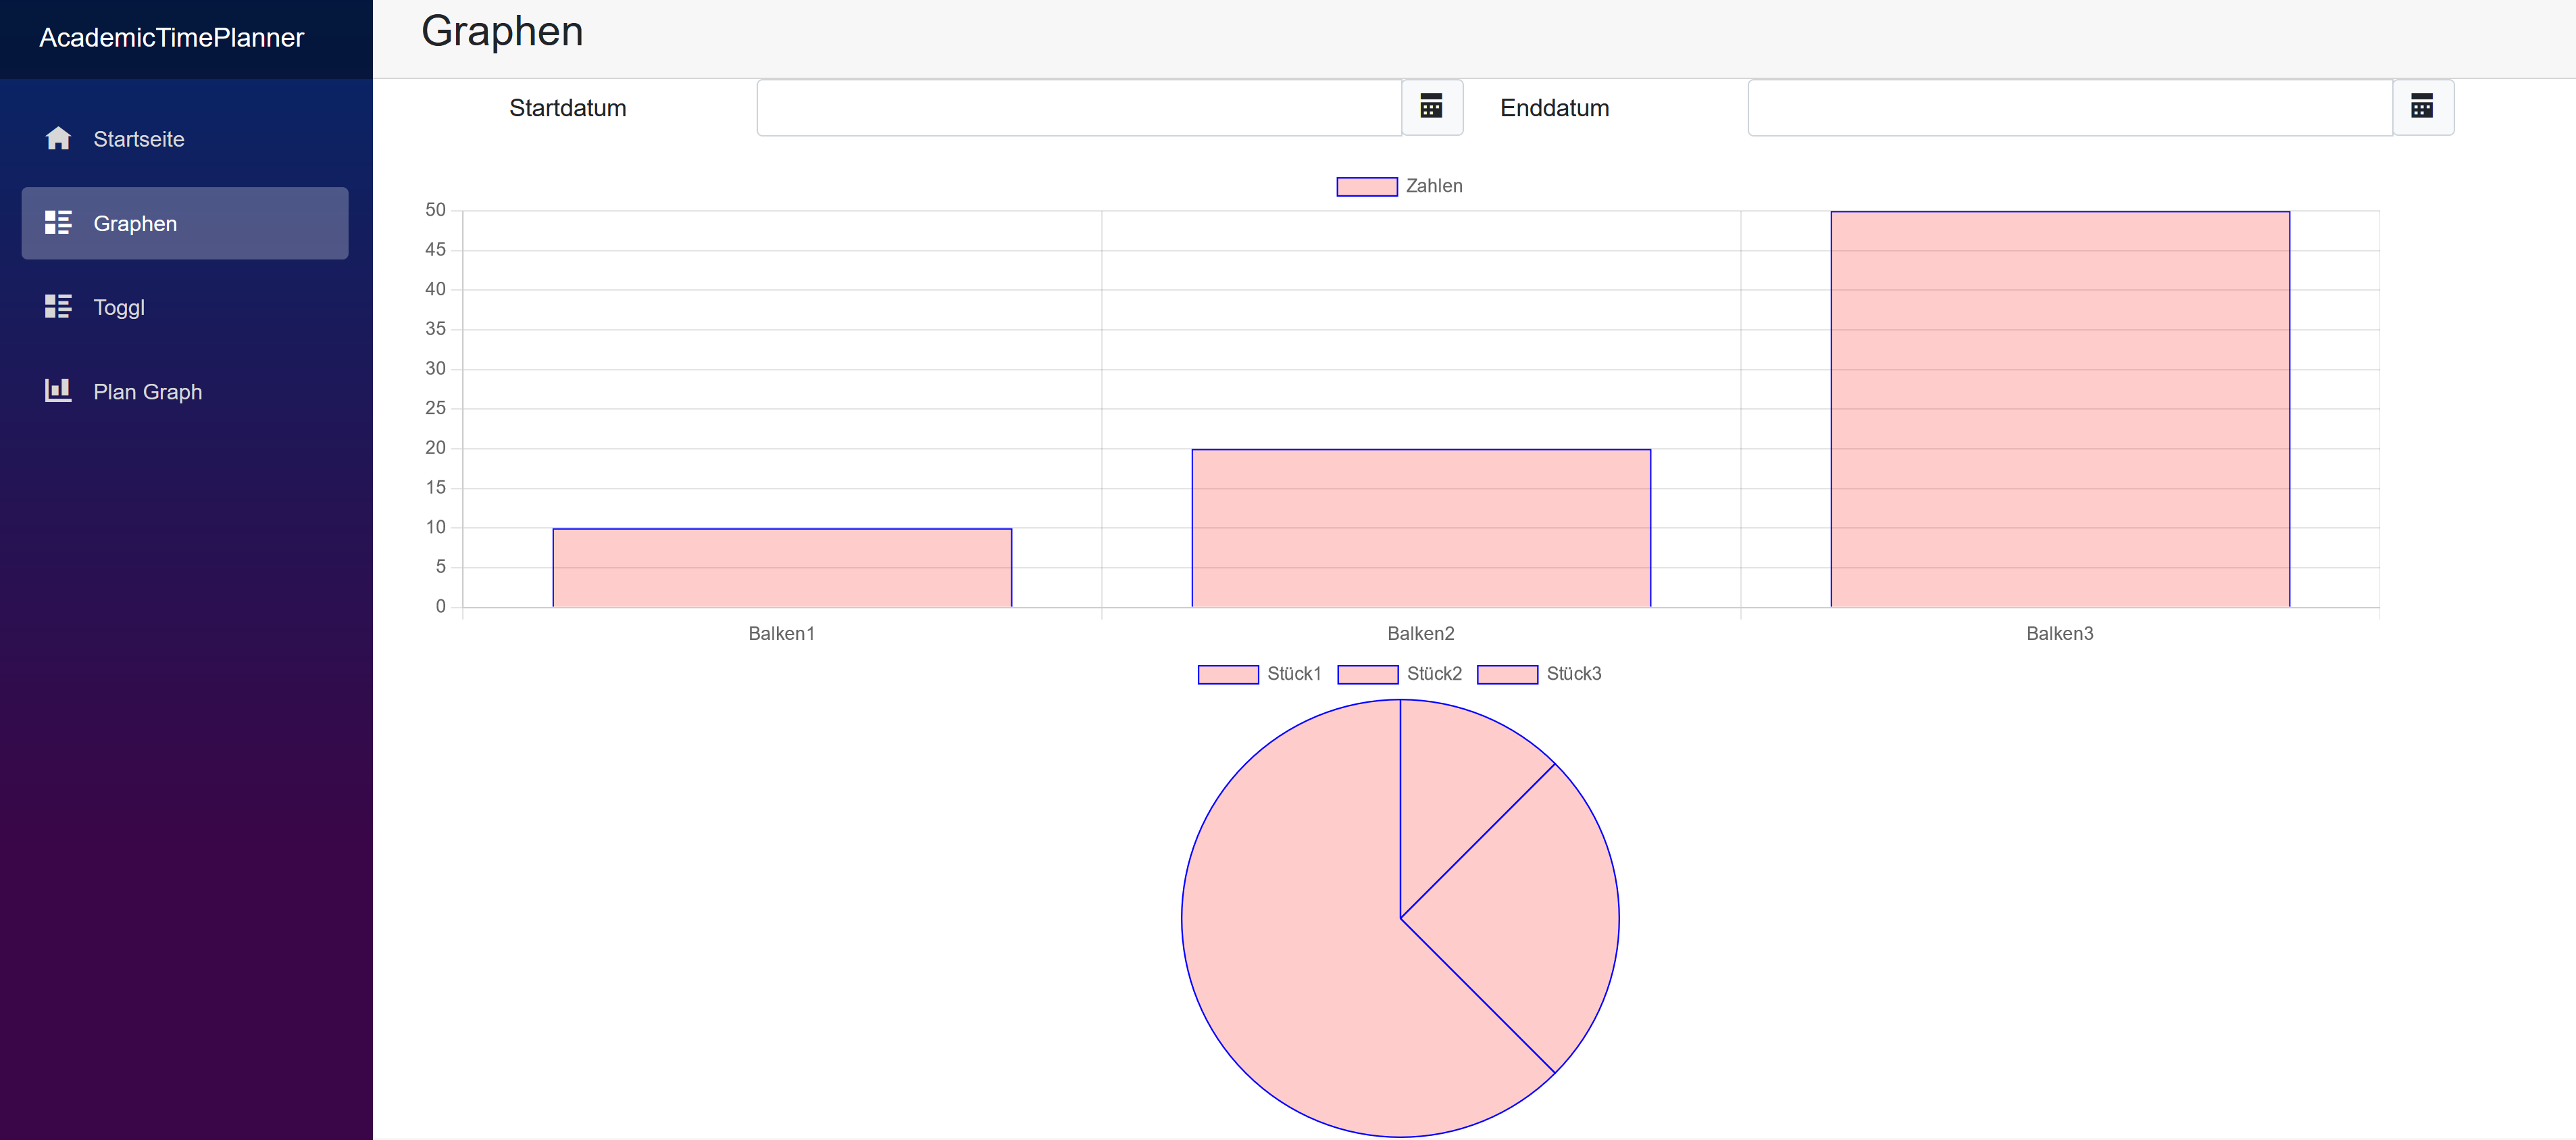
\includegraphics[width=1.0\columnwidth]{figure1_prototype_charts}
\caption{ATP prototype displaying dummy charts}
\label{figure1}
\end{figure}

\section{Toggl Track}
Toggl Track is an easy-to-use, multifunctional online time tracking application. Tasks can be tracked and grouped
into projects. Tracking can be started and stopped using start and stop buttons. Times can also be manually entered
and assigned to a task and a project. Toggl Track offers many additional functionalities including billing and invoicing,
payroll calculating, generation of detailed reports and project budgeting. Toggl Track can be used on different devices 
like computers, smartphones and tablets. The tracking data is then synchronized between the devices. Furthermore, Toggl 
Track provides an API to be used to query tracked time entries from Toggl Track which can then be used outside Toggl Track 
itself, e. g. by other applications. \cite{bachelorarbeit_Egger_Verstappen_page8} \cite{toggl_track_url}

\section{GitHub} \label{GitHub}
GitHub \cite{github_url} is an inline service which provides Git based version control for software projects.
\subsection{Version control}
Version control is used to see what was changed when and by whom. It can also be used to roll back to an older state if needed. In GitHub a feature branch is created to implement a certain feature, and afterwards when finished such a branch will be integrated into the main branch via a pull request. This pull request allows the other members of the team to request changes before the branch is merged into the main branch. This process also enables members of a team to work independently without the problem of accidentally interfering with an other team member's work.
\subsection{GitHub Actions}
GitHub Actions is a (CI/CD) platform \cite{github_actions_url}. It allows for build and test automation as well as maintaining deployment pipeline. Furthermore, workflows to automatically test and build the software on every pull request. This feature helps to prevent the accidental inclusion of broken features or features which ,when isolated work as intended, but would cause other parts of the project to crash when integrated into it.
\subsection{GitHub Issues}
Issues are often related to features and the corresponding feature branches. They provide the possibility to break down a milestone into manageable tasks which can then be assigned to the members of the team to work on. Thus, tasks and their assigned members can be monitored and identified. 
